%=========================================================================
\chapter{Úvod}
Ochrana a~zabezpečení soukromých a~důležitých informací je v~dnešní době často se vyskytujícím
tématem na poli informačních technologií. Ať už se bavíme o~zabezpečení dat při přenosu po síti
nebo o~zabezpečení lokálně uložených dat. Dokážeme si asi představit situaci, kdy potřebujeme
sdílet informace, ale chceme zajistit, že je budou schopny přečíst pouze osoby, které jsou k~tomu
určeny.

 Výše uvedeného lze dosáhnout šifrováním informací. V~dnešní době existuje nespočet možností, jak
informace šifrovat. Kvalitu zabezpečení dat značně ovlivňuje výběr použitého šifrovacího
algoritmu a~dostatečně silného hesla. Pokud použijeme slabou šifru a~silné heslo, je
šance, že se k~Našim datům dostane neoprávněná osoba je výrazně nižší, než když to uděláte naopak.

 Často chceme sdílet nebo zabezpečit více než jeden soubor s~informacemi. Obecně se pro
spojení více souborů různého typu do jednoho celku používají archivy. Jedním z~nejrozšířenějších
typů souborových archivů jsou formáty .ZIP a~.7z.

 Tato práce se převážně zabývá analýzou používaných metod zabezpečení a~šifrovacích
algoritmů u~těchto formátů a~následně získáváním hesel k~takto zabezpečeným souborům. Výsledky
analýz jsou použity pro návrh rozšiřujících modulů nástroje {\it Wrathion}. Práce se také
zabývá přiblížením paralelismu a~problémů s~ním spojených. Jsou zde také popsány základní
principy a~struktury standardu a~frameworku OpenCL.

 V~kapitole \ref{ch:sifrovani} s~podíváme na šifrovací a~hešovací metody používané formáty
archivů. V~kapitole \ref{ch:opencl} si přiblížeme technologii OpenCL, která je použita pro
akceleraci pomocí grafické karty v~nástroji {\it Wrathion}. Ten je popsán v~kapitole
\ref{ch:wrathion}. V~kapitole \ref{ch:formaty} jsou zanalyzovány formáty .ZIP a~.7z. Na základě
poznatků z~analýz jsou v~kapitole \ref{ch:moduly} vytvořeny návrhy rožšiřujících modulů {\it
Wrathionu}. 
\chapter{Metody pro šifrování a~hešování}
\label{ch:sifrovani}
Chceme--li se bavit o~šifrování a~hešování musíme si nejprve definovat pojem \uv{kryptografie}.
\begin{defn}
    \uv{Kryptografie je studie matematických technik spojených s~aspekty bezpečnosti informací jako
    například důvěrnost, integrita dat, ověřování entit a~ověřování původu dat.}~\cite{AC:1996} 
\end{defn}
Pojmy \uv{šifrování} a~\uv{hešování} vyjadřují dva různé přístupy k~zabezpečení informací. Oba pojmy
vyjadřují použití algoritmů nebo funkcí navrhnutých na základě kryptografických pravidel. 
i
\section{Šifrování}
Pokud potřebujeme zabezpečit data tak, aby během přenosu nebyla čtena neoprávněnou osobou, která by
mohla data jakkoliv získat, bavíme se o~šifrování. Pro šifrování potřebujeme heslo, které použijeme
pro zamaskování informací tak, aby původní zpráva nebyla čitelná. V~případě šifrování však
potřebujeme umět data znovu odmaskovat a~tím udělat čitelnými~\cite{AC:1996}. Podle toho rozlišujeme metody na dva
typy:
\begin{itemize}
    \item Symetrické šifry -- pro šifrování i~dešifrování jsou použity stejné klíče (hesla).
        Nejznámější metodou je DES, která byla vytvořena v~roce 1975 společností IBM. Posléze na to
        byla standardizována. V~součastnosti se již skoro nepoužívá, dala ovšem základ dalším
        používaným šifrovacím metodám. Mezi další známé symetrické šifry patří např.: 3DES, AES, RC4
        a~jiné.
    \item Asymetrické šifry -- v~tomto případě je pro šifrování a~dešifrování použit jiný klíč.
        Tento mechanismus našel své uplatnění hlavně v~elektronických podpisech. Ty používají tzv.
        veřejný klíč a~klíč soukromý. Pokud chcemezamaskovat informace použijeme veřejný klíč pro
        šifrování a~soukromý pro dešifrování. Druhá kombinace klíčů slouží k~ověření dat a~k~šifrování.
\end{itemize}

\subsection{Triple Data Encryption Algorithm (TDEA, 3DES)}
Jedná se o~rozšířenou verzi metody
DES\footnote{Specifikace na \url{http://csrc.nist.gov/publications/fips/fips46-3/fips46-3.pdf}}.
K~vytvoření této metody došlo na základě nedostatečné bezpečnosti metody DES proti útokům hrubou
silou. Jedním z~požadavků na novou metodu byla zpětná kompatibilita s~metodou DES tak, aby
společnosti nemusely předělávat své systémy.

TDEA je symetrická bloková šifra využívající kryptografické jádro DES k~šifrování 64-bitového bloku
dat. Metoda pracuje s~64-bitovým klíčem, ovšem pro šifrování je použito pouze 56 bitů, zbylé bity
slouží k~detekci chyb. 

Metoda používá tři 56-bitové klíče pro své operace. Jednotlivé klíče jsou použity v~různých krocích
zpracování vstupních dat. Prováděné kroky jsou:
\begin{enumerate}
    \item šifrování dat pomocí klíče K1,
    \item dešifrování dat pomocí klíče K2,
    \item šifrování dat pomocí klíče K3.
\end{enumerate}
Metoda může být použita v~režimech:
\begin{itemize}
    \item Klíče jsou reprezentovány na 168 bitech a~jsou definovány jako K1 $\neq$ K2, K2 $\neq$ K3
        a~K1 $\neq$ K3. Každý klíč je tedy unikátní.
    \item Klíče jsou reprezentovány na 112 bitech. Zde jsou definovány jako K1 = K3 a~K1 $\neq$ K2.
    \item Posledním režimem je použití jednoho 56-bitového klíče, tedy K1 = K2 = K3.
\end{itemize}
První a~druhý režim jsou jedinými možnostmi schválenými standardem jako dostatečné. Třetí režim
je použit pouze pro kompatibilitu s~DES. Pokud se totiž podíváme na prováděné kroky tak zjistíme,
že pokud jsou všechny klíče identické je výstup TDEA identický s~výstupem DES při použití stejného
klíče~\cite{NIST:2012}.

\subsection{Advanced Encryption Standard (AES)}
Tento standard byl vytvořen kvůli nedostatkům šifrovací metody Triple DES v~síle šifrování a
v~rychlosti šiforvání dat. Původní název této šifrovací metody je Rijndael. Metoda Rijndael byla
vybrána institutem National Institute of Standards and Technology jako nejlépe vyhovující metoda ze
všech přihlášených. Standard byl publikován v~roce 2001~\cite{NIST:2001}.

Jedná se o~symetrickou blokovou šifru používající 128-bitový datový blok s~proměnnou délkou
šifrovacího hesla. Délka hesla může být 128, 192 nebo 256 bitů. To je reflektováno v~názvu metody
(AES-128, AES-192, AES-256). Metoda pracuje s~daty po bajtech, které případně organizuje do polí
nebo dvoudimenzionálních polí bajtů. V~metodě AES je použito dvoudimenzionální pole skládající se
ze čtyř řádků obsahujících čtyři bajty. Toto dvou dimenzionální pole je nazýváno {\it State}.

Na začátku šifrování se nakopírují data ze vstupu do pole {\it State} a~nastaví se
zaokrouhlovací klíče ({\it Round Keys}). Poté je, na základě použité délky šifrovacího klíče, x--krát
použita zaokrouhlovací funkce. Počet opakování funkce je 10-krát pro 128b klíč, 12-krát pro 192b
klíč a~14-krát pro 256b klíč. Funkce se skládá ze čtyř bajtově-orientovaných transformací:
\begin{enumerate}
    \item nahrazení bajtů pomocí nahrazovací tabulky -- nelineární nahrazení bajtů, které funguje
        nezávisle pro každý byte pole {\it State},
    \item posun řádků pole {\it State} o~různou hodnotu (offset) -- je použit cyklický posun
        (rotace) vlevo, kde velikost posunu je rovna indexu řádku pole, tedy 0 až 3,
    \item smíchání dat v~rámci každého sloupce pole {\it State} -- každý sloupec je považován za
        samostatný polynom čtvrté úrovně, nad kterým jsou prováděny operace,
    \item přidání zaokrouhlovacího klíče ({\it Round Key}) k~poli {\it State} -- zaokrouhlovací
        klíče jsou přidávány pomocí bitové operace XOR provedené nad sloupci pole.
\end{enumerate}
Pro dešifrování je použita inverzní funkce, a~protože se jedná symetrickou šifru, je pro dešifrování
použito stejné heslo jako pro šifrování.

\section{Hešování}
Hešování se používá k~jednosměrnému zabezpečení dat. V~tomto případě se nepoužívají hesla pro
zabezpečení dat. Jde o~kombinaci logických funkcí, bitových rotací, posunů a~záměny posloupnosti
bitů. Úkolem těchto metod je na vstupu přijmout zprávu o~jakékoliv veliskosti a~na výstup produkovat
zprávu o~pevné délce. 

 V~případě optimální hešovací funkce nelze pro dvě různé vstupní zprávy obrdžet identické zprávy
výstupní. Toho lze využít pro bezpečné uložení informací, které není nutné někdy v~budoucnosti
převést do původního stavu. Těchto vlastností se využívá například při ukládání hesel nebo
ověřování, zda nedošlo při přenosu k~modifikaci dat. Do této skupiny patří funkce: MD4, MD5, SHA-1,
SHA-2 a~jiné~\cite{AC:1996}.

\subsection{SHA-1}
Slouží pro hešování zpráv s~maximální délkou $2^{64}-1$ bitů. Jako výstup produkuje 160 bitovou
hodnotu tzv. heš (hash). Ten je většinou uveden v~hexa-decimální formě pro snížení nároků na uložení
a vizuálního zkrácení výstupu~\cite{NIST:2015}. 

Existují dvě možnosti, jak vytvořit výstupní hodnotu. Jedna vyžaduje více zdrojů, ale ve většině
případů potřebuje kratší výpočetní čas. Druhá se spíše hodí
pro systémy s~omezenými zdroji, které nevyžadují co nejrychlejší zpracování.


\subsection{SHA-256}
Nástupce SHA-1, mající stejná omezení pro vstupní zprávu jako jeho předchůdce, se však liší v~délce
výstupní hodnoty, která má v~tomto případě velikost 256-bitů. To poskytuje podstatně víc možných
vypočtených hodnot a~sníží se tedy procentuální pravděpodobnost, že dojde ke kolizi vypočtených
hodnot pro různé vstupní zprávy, což se používá jako jeden z~možných útoků na hešovací
funkce~\cite{NIST:2015}.

Tato hešovací funkce má taktéž vyšší nároky na zdroje při výpočtu výsledku. Nemá takové paměťové
nároky jako její předchůdce. Avšak výpočet je realizován pomocí šesti logických funkcí namísto
původních čtyř. Tím se prodlužuje čas potřebný k~získání výsledku.

%\begin{algorithm}[ht]
%    \SetStartEndCondition{ (}{)}{)}\SetAlgoBlockMarkers{}{}%
%    \SetKwProg{Fn}{}{\string:}{}%
%    \SetKwFor{For}{for}{\string:}{}%
%    \SetKwIF{If}{ElseIf}{Else}{if}{}{else if}{else}{}%
%    \SetKwFor{While}{while}{}{}%
%    \SetKwRepeat{Repeat}{repeat}{until}%
%    \SetKwInOut{Input}{vstup}\SetKwInOut{Output}{výstup}
%    \AlgoDisplayBlockMarkers\SetAlgoNoLine%
%    \DontPrintSemicolon
%    \Input{Zpráva $M$ o~délce $l$, kde $0 < l \leq  2^{64}$ bitů}
%    \Output{Heš o~délce 160--bitů}
%    \Fn{SHA-1 ($M$)}{
%        Zarovnej zprávu, aby výsledek byl násobkem $512$\;
%        Rozděl nově vytvořenou zprávu na $N$ bloků po $512$ bitech ($16 * 32$ bitů blok)\;
%        Nastavení výchozích hodnot hešů $H^{(0)}_i$, kde $i = \{0,4\}$\;
%        \For{$i = 1;\,i < N;\,i = i~+ 1$}{
%            $W = f_{rozsir}(B)$ \tcc*[r]{z $ 16 * 32$-bit hodnoty na $80 * 32$-bit hodnotu}
%            \tcp*[l]{Inicializuj registry konstantami}
%            $a = H_0,\,b = H_1,\,c = H_2,\,d = H_3,\,e = H_4$\;
%            \For{$t = 0;\, t < 80;\, t = t + 1$}{
%                $s = t \wedge MASK$\;
%                \If{$ t \geq 16$}{
%                    $W_s = ROTL^1(W_{(s+13)\wedge MASK} \oplus W_{(s+8)\wedge MASK} \oplus
%                    W_{(s+2)\wedge MASK} \oplus W_s$\;
%                }
%                \If{$ 0 \leq i~\leq 19$}{
%                    $T = ROTL^5(a) + (x \wedge y) \oplus (\neg x \wedge z) + e + K_t + W_s$\;
%                }
%                \ElseIf{$20 \leq i~\leq 39$ or $60 \leq i~\leq 79$}{
%                    $T = ROTL^5(a) + (x \oplus y \oplus z) + e + K_t + W_s$\;
%                }
%                \ElseIf{$40 \leq i~\leq 59$}{
%                    $T = ROTL^5(a) + (x \wedge y) \oplus (x \wedge z) \oplus (y \wedge z) 
%                        + e + K_t + W_s$\;
%                }
%                $e = d, d = c$\;
%                $c = ROTL^{30}(b)$\;
%                $b = a, a~= T$\;
%            }
%            $H^{(i)}_0 = a~+ H^{(i-1)}_0$\;
%            $H^{(i)}_1 = b + H^{(i-1)}_1$\;
%            $H^{(i)}_2 = c + H^{(i-1)}_2$\;
%            $H^{(i)}_3 = d + H^{(i-1)}_3$\;
%            $H^{(i)}_4 = e + H^{(i-1)}_4$\;
%        }
%        \Return{$concat(H^{(N)}_0, H^{(N)}_1, H^{(N)}_2, H^{(N)}_3, H^{(N)}_4)$}
%    }
%
%    \caption{Princip funkce SHA1} \label{alg:SHA}
%\end{algorithm}

\chapter{Paralelní výpočty na GPU pomocí OpenCL}
\label{ch:opencl}
Dnešním trendem ve vývoji architektur pro výpočetní zařízení je umožnění paralelního provádění
úloh. Jedná se o~architektury otevírající dveře k~znatelnému zvýšení výkonu u~zařízení na nich
postavených. Dnes již považujeme za normální, že máme více jádrové procesory (CPU), které
podporují paralelní zpracování. Ovšem jedním z~hlavních představitelů toho trendu jsou grafické 
výpočetní jednotky (GPU). Existence těchto typů zařízení ústí v~potřebu mít prostředkya, jak s~těmito
zařízeními komunikovat a~programovat je.

 U~paralelních aplikací je naší největší prioritou efektivnost využití zdrojů. Důvodem je
vysoká pořizovací cena a~často i~vysoké provozní náklady. Dalším důvodem je také náročnost aplikací
na nich běžících. Ty jsou ve většině případů časově velmi náročné. Návrh i~programování aplikace
využívající paralelismů může být značně náročné. Je zde velký rozdíl v~programovacích technikách.
Programování paralelních aplikací pro CPU vychází ze zažitých standardů pro práci s~pamětí,
procesy nebo pro řízení běhu aplikace, používaných pro vývoj klasických aplikací. Oproti tomu
programování GPU a~jiných specializovanějších zařízení se od těchto standardů velmi liší.
Například vytváření obecně použitelné aplikace určené pro běh na GPU je náročné hlavně z~hlediska
odlišného paměťovému modelu a~jiné škály funkcí pro práci s~ní. GPU ve značné míře využívá
operace pro práci s~vektory. Největším problémem spojeným s~programováním těchto zařízení je škála
různých používaných architektur. Faktem je, že všechny modely pro práci se zařízeními (paměťový
model, model provádění atd.) se mohou měnit v~závislosti na platformě, výrobci či použitím
hardwaru.

 Takovýto vývoj obecně použitelných aplikací by byl nereálný, protože bychom museli
aplikaci vyvinout v~desítkách ne--li stovkách verzí pro jednotlivá konkrétní zařízení, na kterých
bychom chtěli aplikaci provozovat. Proto se vyskytla potřeba vytvořit univerzální rozhraní, jež by
nad specifickými přístupy k~programování jednotlivých zařízení vytvořilo univerzální programovací
vrstvu, jejíž instrukce by následně byly interpretovány do instrukční sady specifického zařízení.
Takovýmto rozhraním je např.: CUDA\footnote{Platforma vyvinutá společností NVIDIA určená pro
umožnění práce s~GPU této společnosti~\cite{NVIDIA}.} nebo OpenCL~\cite{AMD:2011}.

\section{OpenCL}
Jedná se o~otevřený nezpoplatněný standard sloužící k~zjednodušení a~zefektivnění programování
paralelních aplikací. OpenCL využívá rozhraní, které pracuje na velmi nízké úrovni, tedy skoro na
úrovni samotných fyzických součástek, čímž dosahuje vysoké efektivity. Nad tímto rozhraním následně
vytváří vrstvu pro výpočty, jenž obsahuje pracovní prostředky nezávislé na platformě. Hlavní síla
OpenCL je zkombinování paralelních výpočtů aplikace na GPU se zřetězeným rendrováním grafických
prvků~\cite{Khronos:2015}.
Standard:
\begin{itemize}
    \item Podporuje datově i~úlohově založené paralelní programovací modely.
    \item Definuje konzistentní numerické požadavky vycházející z~IEEE 754.
    \item Definuje konfigurační profil pro přenosná zařízení a~vestavěné systémy.
    \item Zajišťuje efektivní součinnost s~OpenGL, OpenGL SE a~dalšími grafickými
        rozhraními.
\end{itemize}
Nejedná se pouze o~standard pro psaní paralelních aplikací, ale i~o~stejnojmenný framework, který
je na tomto standardu postaven. Framework OpenCL zahrnuje programovací jazyky, rozhraní pro
programování aplikací (API), knihovny a~systém pro běh programu ({\it runtime} systém).
\subsection{Architektura OpenCL}
Struktura OpenCL architektury lze popsat hierarchickým modelem následovně:
\begin{itemize}
    \item model platformy,
    \item model provedení,
    \item model paměti,
    \item programovací model.
\end{itemize}

\subsubsection{Model platformy}
Tento model se skládá z~hostitele a~jednoho nebo více OpenCL zařízení, která jsou rozdělena na
jedno nebo více výpočetních jednotek. Ty jsou dále děleny na jeden nebo více výpočetních prvků.
Na jednotlivých prvcích se pak provádí výpočetní operace.

 Rozdělení na hostitele a~zařízení vyžaduje implementovat aplikaci pro obě části. Tedy
vytvořit kód pro hostitele a~kód pro GPU zařízení ({\it OpenCL kernel}). Vezmeme--li si jako
příklad standardní počítač tak hostitel je CPU a~zařízení je GPU, případně více GPU.
\begin{figure}[ht]
    \begin{center}
	\scalebox{0.3}{
	    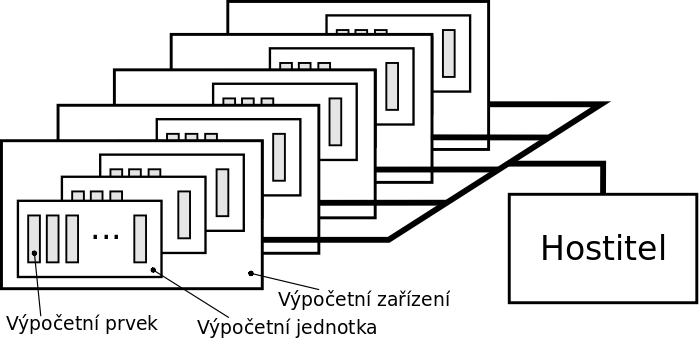
\includegraphics{fig/opencl_platform_model}
	}
    \end{center}
    \caption{Model OpenCL platformy \cite{Khronos:2015}}
    \label{platform}
\end{figure}
\subsubsection{Model provedení}
Jak již bylo zmíněno aplikace se dělí na dvě části. Zde hovoříme o~kernelech a~o~hostitelově
programu, přičemž kernel je ten, kdo provádí výpočty. Tato \uv{práce} je prováděna pomocí
pracovních položek ({\it work-item}) jenž můžeme sdružovat do pracovních skupin ({\it
work-group}).

 Hostitel má za úkol spravovat kontext aplikace a~na jeho základě nastavit prostředí, ve
kterém bude kernel provádět operace. V~prostředí musíme specifikovat a~nastavit tyto položky:
\begin{itemize}
    \item Zařízení -- jedno a~více zařízení ovladatelných platformou OpenCL.
    \item Objekty kernelu -- OpenCL funkce s~přednastavenými argumenty podle vybraného
        zařízení.
    \item Objekty programu -- zdrojový kód a~jeho spustitelná verze, které implementují
        kernely.
    \item Objekty paměti -- proměnné, ke kterým může přistupovat hostitel i~OpenCL zařízení.
	Instance kernelů během svého provádění operují s~těmito objekty.
\end{itemize}
Hostitel se zařízením komunikuje pomocí front příkazů, do nichž se příkazy rozřadí podle
typu operace. Jednotlivé příkazy ve frontě se provádí relativně k~ostatním příkazům. Pořadí
provádění může být definováno následujícími modely:
\begin{itemize}
    \item {\it In-order} -- příkazy se provádí a~mají efekt tak, jak do fronty přišly.
    \item {\it Out-of-order} -- pořadí provedení příkazů je omezeno pouze explicitně uvedenými
        synchronizačními body nebo explicitně definovanými závislostmi na událostech.
\end{itemize}

\subsubsection{Model paměti}
Práce s~pamětí v~OpenCL se značně liší od klasického přístupu, který známe ze standardních
aplikací určených pro běh pouze na CPU. Paměťový model OpenCL popisuje obsah, strukturu a~chování
paměti používané v~platformě vytvořené tímto frameworkem.

 Pro každou aplikaci je třeba přesně definovat, jak přesně bude její paměť vypadat.
Model dělíme na čtyři části:
\begin{itemize}
    \item {\it Oblasti paměti} -- definuje, se kterými oblastmi paměti hostitel a~zařízení ve
	stejném kontextu mohou pracovat.
    \item {\it Objekty paměti} -- jsou definované v~OpenCL API, o~správu se stará hostitel i
	zařízení.
    \item {\it Sdílenou virtuální paměť} -- jedná se o~virtuální adresový prostor přístupný oběma
	částem aplikace.
    \item {\it Model konzistence} -- definuje pravidla pro oblasti paměti, které jsou používané
	více jednotkami naráz a~zaručuje, že je dodrženo pořadí operací s~pamětí a~že jsou data po
	celou dobu validní. Taktéž definuje synchronizaci nad těmito oblastmi.
\end{itemize}
Pro nás je nejdůležitější pochopit, jak je paměť strukturována a~jak na sebe navazují
jednotlivé oblasti. To je nejlépe patrné z~obrázku \ref{memory}. Popis struktury:
\begin{itemize}
    \item paměť hostitele (RAM apod.),
    \item paměť zařízení,
    \begin{itemize}
	\item {\it globální paměť} -- oblast je přístupná pro čtení i~zápis všem jednotkám
v~kontextu nezávisle na zařízení,
	\item {\it paměť konstant} -- před zahájením výpočtu je alokovaná a~inicializována
	    hostitelem a~v~průběhu výpočtu se tato oblast nemění výpočtu,
	\item {\it lokální paměť} -- oblast je přístupná všem pracovním položkám ve
	    stejné pracovní skupině,
	\item {\it soukromá paměť} -- oblast je přístupná pouze jedné pracovní položce.
    \end{itemize}
\end{itemize}
\begin{figure}[ht]
    \begin{center}
	\scalebox{0.3}{
	    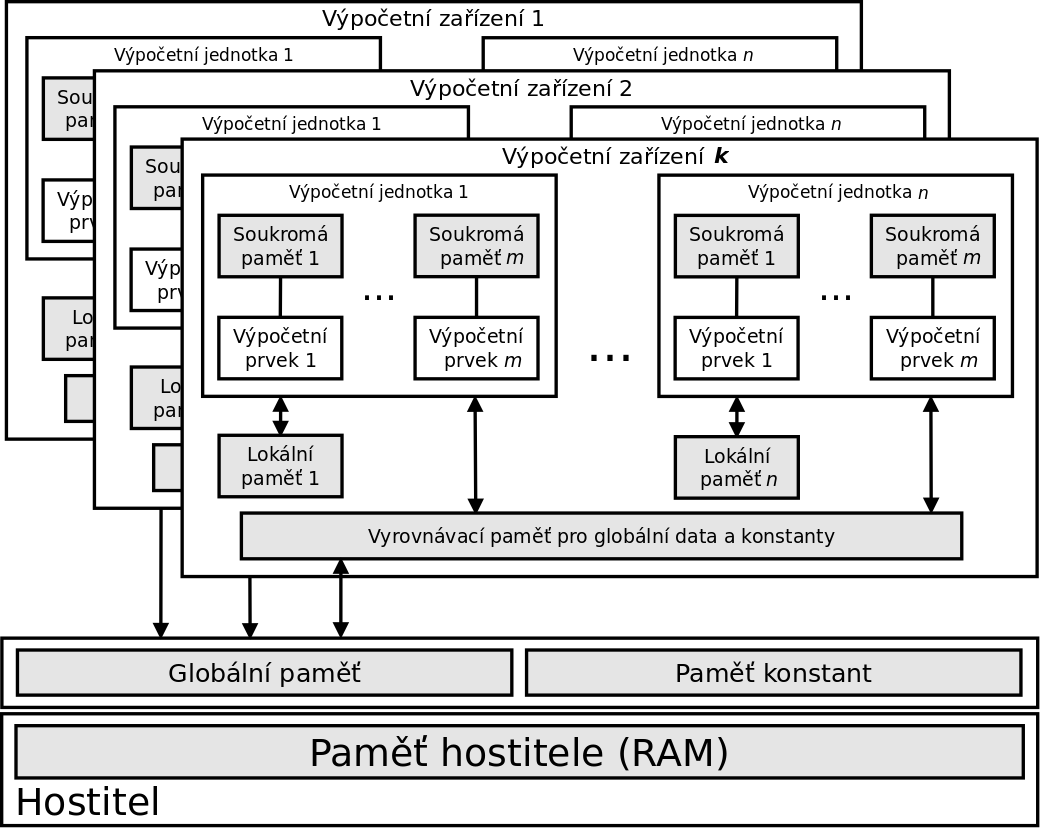
\includegraphics{fig/opencl_memory_structure}
	}
    \end{center}
    \caption{Struktura paměti OpenCL \cite{Khronos:2015}}
    \label{memory}
\end{figure}
\subsubsection{Programovací model}
Tento model lze také nazvat jako OpenCL framework. Framework se skládá ze třech komponentů. Zde za
zmínku stojí OpenCL kompilátor. Ten podporuje pokročilý jazyk SPIR-V a~jazyk OpenCL C. Další
jazyky mohou být podporovány některými implementacemi kompilátoru.


\chapter{Nástroj Wrathion}
\label{ch:wrathion}
Jedná se o~nástroj vytvořený Janem Shmiedem v~roce 2014 v~rámci jeho diplomové
práce~\cite{Schmied}. Nástroj byl vytvořen pro použití v~projektu {\it Moderní prostředky pro 
boj s~kybernetickou kriminalitou na Internetu nové generace, MV, VG20102015022}.
\section{Hlavní části Wrathionu}
Nástroj slouží ke obnovování hesel pomocí brute-force útoků na tato hesla. Skládá se ze tří
částí:
\begin{itemize}
	\item jádra -- zprostředkovávajícího funkcionalitu potřebnou pro crackování,
	\item modulů -- skrze které je zajištěna podpora crackování různých formátů,
	\item aplikace -- umožňující pracovat s~frameworkem a~moduly pomocí CLI rozhraní.
\end{itemize}
\begin{figure}[ht]
    \begin{center}
	\scalebox{0.34}{
	    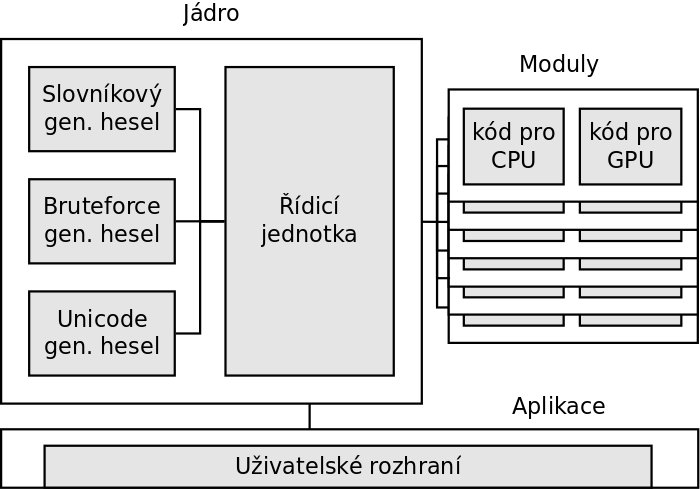
\includegraphics{fig/wrathion_structure}
	}
    \end{center}
    \caption{Schéma struktury nástroje Wrathion \cite{Hranicky}}
    \label{memory}
\end{figure}
\subsection{Generátory hesel}
První částí Wrathionu, kterou si rozebereme jsou generátory hesel pro útoky. Jedná se o~esenciální
funkcionalitu. Bez vygenerovaných hesel nemůžeme na útoky vůbec myslet. V~nástroji jsou momentálně
implementovány tři typy generátorů:
\begin{itemize}
    \item {\it Brute-force} -- postupně generuje všechny možné permutace ze zadaných znaků.
    \item {\it Unicode} -- jedná se o~upravený brute-force generátor. V~tomto případě je nastavena
	vstupní abeceda na všechny Unicode znaky a~z~nich jsou generovány možné permutace hesel.
    \item {\it Rule-based} -- velmi podobný předchozím variantám ovšem umožňuje specifikovat různá
	podpůrná pravidla pro generování hesel. Například, že má být první písmeno velké, druhé má
	být 'a' a~že poslední 2 znaky jsou číslice. Toto umožňuje zúžení počtu permutací a~tedy
	snižuje čas potřebný k~vygenerování všech jejich variant (tento typ generátoru je teprve
	ve vývoji).
    \item {\it Dictionary} -- slovníkový generátor, který využívá externí soubory s~často
	používanými hesly.
\end{itemize}
Nejčastěji používaným generátorem je brute-force, který je ovšem výpočetně náročný. Jedná se
však o~snadno paralelizovatelný generátor, proto je příhodně implementován i~jako kernel běžící na
GPU.
\subsection{Crackery}
Druhou částí jsou samotné crackery, které dělíme podle toho, kdo provádí generování hesel a
kdo provádí porovnávání hesel:
\subsubsection{CPU cracker}
Zde se standardně spustí již předkompilovaný cracker napsaný v~C++ (viz. Obrázek \ref{CPU}). Není
zde žádný větší problém s~generováním ani následným ověřováním hesel, ovšem výpočetní síla
u~paralelizovatelných algoritmů není CPU ani zdaleka tak vysoká jako na GPU. Proto, pokud je to
možné, volíme druhou variantu crackeru.
\begin{figure}[ht]
    \begin{center}
	\scalebox{0.3}{
	    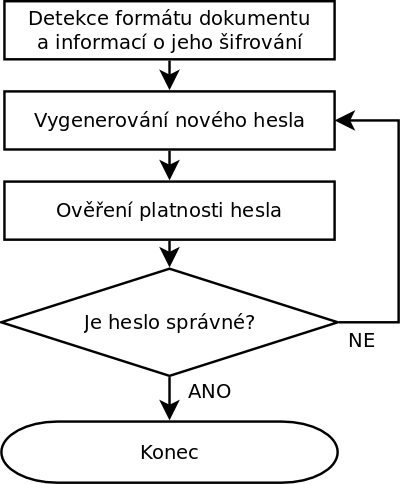
\includegraphics{fig/proces}
	}
    \end{center}
    \caption{Proces generování a~ověřování hesel na CPU \cite{Schmied}}
    \label{CPU}
\end{figure}

\subsubsection{GPU cracker}
Cracker může pracovat ve dvou režimech (viz. Obrázek \ref{CPUGPU}). V~prvním hesla generujeme na
CPU a~pak je posíláme do paměti GPU, kde jsou crackerem zpracována. To má ovšem velkou nevýhodu
v~tom, že musíme pořád posílat data z~paměti hostitele (CPU) do privátní paměti výpočetního prvku
(výpočetní jednotka na GPU).
\begin{figure}[ht]
    \begin{center}
	\scalebox{0.32}{
	    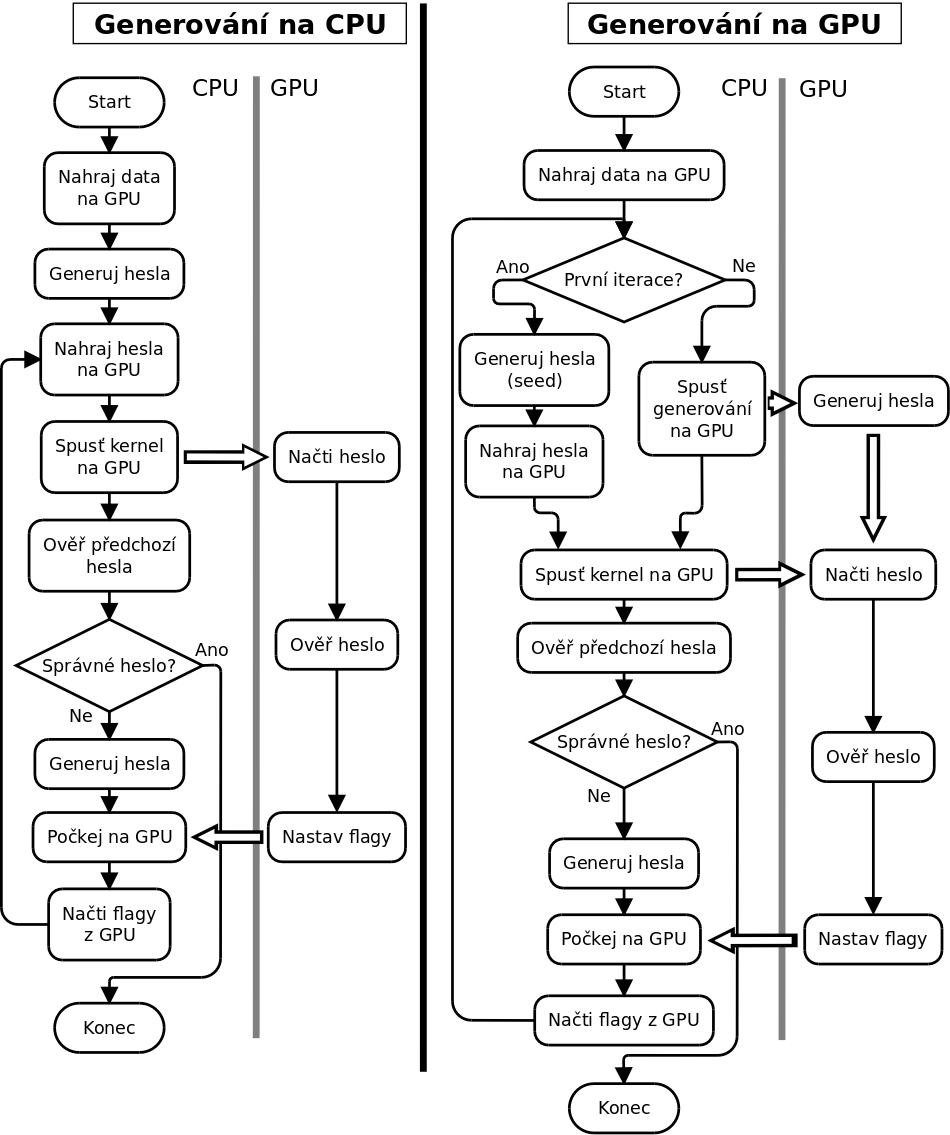
\includegraphics{fig/generators}
	}
    \end{center}
    \caption{Proces generování hesel na CPU a~ověřování na GPU \cite{Schmied}}
    \label{CPUGPU}
\end{figure}

 Druhou a~efektivnější možností je generovat hesla přímo na GPU do privátních pamětí čím
minimalizujeme množství dat, které musí putovat od hostitele k~zařízení. Tímto snížíme výslednou
prodlevu výpočtů.

 V~obou případech je nutné před zahájením jakýchkoliv operací GPU
 inicializovat\linebreak OpenCL systém. Tedy vytvořit kontext, fronty příkazů, zajistit načtení a
 přeložení požadovaného kernelu a~až poté nahrát nebo vygenerovat data do/na GPU.

\subsection{Moduly}
Nástroj je navržen s~velkým důrazem na modularitu. V~současné době obsahuje pouze tři moduly.
Další moduly pro Wrathion jsou ve fázi vývoje.

\subsubsection{Modul ZIP}
V~této práci nás nejvíce zajímá modul ZIP. Ten v~původním návrhu obsahuje pouze šifrování
obnovování hesel z~archivů šifrovaných algoritmy PKZIP, AES-128, AES-192, AES-256, což zanechává
prostor pro implementaci dalších, formátem {\it .ZIP}, podporovaných metod. Zajímavostí je, že
tento modul byl schopný v~době svého vzniku obnovit heslo šifrovaných {\it .DOCX} souborů, avšak
tento nedostatek u~zabezpečení formátu {\it .DOCX} byl později odstraněn a~tento modul již tedy
není schopen obnovit heslo u~souborů vytvořených po zmíněné aktualizaci.

\subsubsection{Modul DOC}
Další modul pracuje s~formátem {\it .DOC}, který byl pokládán za základní formát aplikace MS Word
z~balíku MS Office. Tento formát byl s~příchodem MS Office 2007 nahrazen formátem {\it .DOCX}.
Nástroj ve své původní podobě obsahuje pouze podporu pro {\it .DOC} formát. Tvorba modulů pro
novější formát {\it .DOCX} spolu s~formáty používanými v~jiných aplikacích balíku MS Office je ve
fázi vývoje.

\subsubsection{Modul PDF}
Prozatím poslední vytvořený modul pracuje s~formátem {\it .PDF}. Zde jsou již implementovány
bezpečnostní revize 1-5. Nástroj počítá i~s~implementací revize 6. Vývoj této funkcionality může
být započat až po zveřejnění specifikace této revize.

\chapter{Analýza formátů .ZIP a~.7z}
\label{ch:formaty}
\section{Formát .ZIP}
Jedná se o~jeden z~prvních formátů souborových archivů, který podporoval kompresi dat. V~roce 1989
vytvořil Phil Katz program PKZIP v~rámci něhož byl představen nový formát .ZIP. Specifikace
formátu .ZIP byla publikována pod veřejnou doménou. Tímto krokem pomohl formátu se stát
celosvětovým otevřeným standardem~\cite{PKWARE:2015}. V~roce 2015 byl formát, ve své specifikaci
6.3.3 z~roku 2012, přijat Mezinárodní organizací pro normalizaci (ISO) a~Mezinárodní
elektrotechnickou komisí (IEC) jakožto standard definovaný dokumentem ISO/IEC
21320-1:2015~\cite{ISOIEC:2015}.

 Formát podporuje velké množství různých komprimačních algoritmů: Store(bez komprese),
UnShrinking, Expanding, Imploding, Tokenizing, Deflating, Enhanced Deflating, BZIP2, LZMA, WavPack
a PPMd~\cite{PKWARE:2014}. 

 Obdobně je to i~s~podporou různých šifrovacích algoritmů:
\begin{itemize}
    \item {\it PKWARE šifrování} -- prvotní šifrování,
    \item {\it DES, 3DES(112-bit a~168-bit)} -- podporováno od verze 5.0 z~roku 2002,
    \item {\it RC2 (40-bit, 64-bit a~168-bit)} -- podporováno od verze 5.0 z~roku 2002,
    \item {\it RC4 (40-bit, 64-bit a~168-bit)} -- podporováno od verze 5.0 z~roku 2002,
    \item {\it AES (128-bit, 192-bit a~256-bit)} -- podporováno od verze 5.2 z~roku 2003.
\end{itemize}
Nastává zde ale problém, že žádný z~ať už volně dostupných nebo komerčních nástrojů
neumožňuje vytvoření archivů se šifrováním DES, RC2 a~RC4. Z~toho tedy plyne, že pravděpodobnost
výskytu archivů šifrovaných těmito metodami je minimální respektive téměř nulová.

\subsection{Struktura souboru}
\label{ssec:zip_struct}
Archivy jsou soubory obsahující další soubory. Dá se tedy říct, že se jedná
o~jakési\linebreak\uv{schránky}, do nichž lze vkládat, ale i~vybírat, určité soubory různých typů.
U~formátu .ZIP lze do archivů navíc ukládat i~adresáře a~tak ukládat
celé struktury tvořené z~adresářů a~souborů \ref{zipstruct}.

\begin{figure}[ht]
    \begin{center}
	\scalebox{0.225}{
	    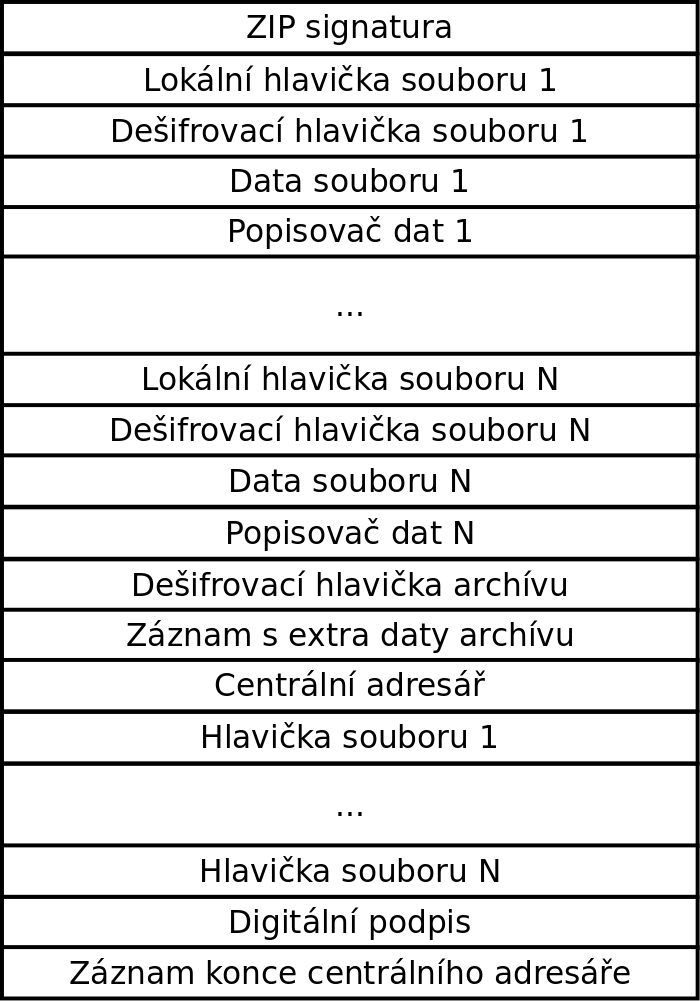
\includegraphics{fig/zip_structure}
	}
    \end{center}
    \caption{Struktura .ZIP souboru \cite{PKWARE:2014}}
    \label{zipstruct}
\end{figure}

 Obsah souboru archivu lze pro lepší orientaci rozdělit na část obsahující definice a~data
uložených souborů a~na část reprezentující organizaci adresářů a~souborů.
\begin{itemize}
    \item První část obsahuje záznamy, jenž se opakují pro každý uložený soubor. Jeden takovýto
záznam musí obsahovat alespoň lokální hlavičku souboru a~data souboru. Pokud je nastaven
3. bit položky {\it General purpose bit flag} v~lokální hlavičce souboru tak musíme ještě počítat
s~tím, že za data byla přidána sekce {\it Data description} o~velikosti 12 bajtů.
    \item Druhá část se skládá ze struktury hlaviček centrálního adresáře (Central Directory
Header). Počet těchto hlaviček odpovídá počtu adresářů a~souborů obsažených v~tomto
archivu. Hlavička centrálního adresáře začíná signaturou [0x50, 0x4b, 0x01, 0x02], podle které je
v~souboru identifikovatelný začátek hlavičky. Za ní následují metadata souboru. Např.: datum a~čas
poslední úpravy obsaženého souboru, velikost před a~po kompresi atd. Tato struktura hlaviček je
ukončena záznamem konec centrálního adresáře. Ten začíná signaturou [0x50, 0x4b, 0x05, 0x06]
a~obsahuje informace o~tom na kterém disku je soubor uložen, na kterém disku začíná struktura
centrálního adresáře a~další.
\end{itemize}
Od verze formátu 6.2 jsou před hlavičkou centrálního adresáře další položky a~to hlavička
pro dešifrování archivu a~záznam o~extra datech archivu. Tyto položky byly přidány
v~závislosti na přidání nové funkce pro šifrování obsahu hlaviček centrálního adresáře.

\subsubsection{Řídící struktury definující šifrování}
 Zatím jsme se bavili pouze o~základní struktuře archivu. Nás ale spíše zajímají struktury
archivů, jenž obsahují soubory v~zašifrované podobě. Zda je soubor šifrován lze zjistit z~jeho
lokální hlavičky nebo z~jeho hlavičky centrálního adresáře a~konkrétně z~prvního a~sedmého bitu
položky {\it General Purpose Bit Flag}. Nastavení prvního bitu indikuje, že je soubor šifrován.
\begin{itemize}
    \item Pokud platí, že není zároveň nastaven i~sedmý bit, je za lokální hlavičku souboru
        přidána hlavička šifrování. Hlavička šifrování se váže pouze k~šifrování pomocí tradiční
        metody od společnosti PKWARE.
    \item Pokud je nastaven i~sedmý bit indikující použití takzvaného \uv{silného
	šifrování}, hlavička šifrování se negeneruje, ale přidávají se informace o~šifrování do
        hlavičky centrálního adresáře a~generuje se záznam s~hlavičkou pro dešifrování, jehož
	část se tváří jako součást dat souboru a~nachází se na samém počátku šifrovaných dat
	souboru.
\end{itemize}
Informace o~metodě šifrování, délce klíče atd., jsou uvedeny v~druhé části souboru
z~důvodů vyšší bezpečnosti. Přesněji v~položce {\it Extra Fields} v~hlavičce centrálního adresáře
příslušící souboru. Položku {\it Extra Fields}, poznáme podle její signatury, kterou začíná a~má
hodnotu [0x00, 0x17]. Další položky obsahují informace o~použitém šifrovacím algoritmu, délce
klíče pro šifrování a~pole příznaků {\it Flags} definující, zda je archiv šifrovaný, jaká je
použita kompresní metoda, co je vyžadováno pro dešifrování, zda je vyžadováno pouze heslo nebo
pouze certifikát nebo je možné použít buď heslo, nebo certifikát. Další možnosti závisí na použitém
certifikátu.

 Záznam pro dešifrování obsahuje o~inicializační vektor (IV, sůl), identifikátor algoritmu pro
dešifrování, bitovou délku šifrovacího klíče, zašifrovaný vzorek náhodných dat (Erddata) a~hlavně
o~informace pro validaci hesla (VData) a~CRC-32 (VCRC32)\footnote{{\it Cyclic Redundancy Code} -
speciální hešovací funkce sloužící pro detekci chyb / změn dat oproti původní hodnotě} těchto
validačních dat. 

\section{Formát .7z}
\label{sec:7z}
Vznik tohoto formátu se datuje do roku 1999 a~jeho autorem je Igor Pavlov. Stejně jako aplikace
7-Zip a~nástrojů spojených s~tímto formátem (7-Max, 7-Benchamark). Formát taktéž slouží
k~vytvoření souborových archivů podobně jako .ZIP. Formát se proslavil hlavně svojí otevřeností a
modulární strukturou. Ta umožňuje skládání libovolných kompresních, konverzních a~šifrovacích
metod.

 Mezi podporované kompresní metody se řadí LZMA, LZMA2, PPMD, BCJ, BCJ2, BZip2 a
Deflate. Jako výchozí metoda je brána LZMA. Hlavní výhody této metody jsou~\cite{7z:2015}:
\begin{itemize}
    \item vysoký kompresní koeficient,
    \item proměnná velikost slovníku,
    \item malé nároky na paměť při dekompresi,
    \item podpora zpracování pomocí multi-threading a~hyper-threading.
\end{itemize}
Další výhodou formátu je podpora komprese velkých souborů, názvy souborů v~Unicode
kódování, možnost spojení více souborů do jednoho toku, který je pak teprve komprimován, komprese
a šifrování hlaviček archivů a~další.

 Standardně použitou šifrovací metodou je AES-256 vyžadující 256-bitové šifrovací heslo.
Takovéto heslo se vytváří pomocí hešovací funkce SHA-256 z~uživatelem zadaného hesla. Pro ještě
vyšší zabezpečení je provedeno \(2^{19}\) iterací při každém vytváření hesla. To může mít na
slabších zařízeních za následek znatelnou prodlevu, než začne komprese souborů a~šifrování.

\subsection{Struktura souboru}
\label{ssec:7z_struct}
Neprázdný soubor tohoto formátu má čtyři části, které v~něm musí být obsaženy viz.
\ref{7zstruct}. Jedná se o~položky: 
\begin{itemize}
    \item První část se nachází hned začátku souboru a~jedná se o~hlavičku se signaturou ({\it
	7zSignature}) ['7', 'z', 0xBC, 0xAF, 0x27, 0x1C] definující začátek souboru daného typu.
	Za ní v~rámci stejné hlavičky jsou informace o~verzi archivu, CRC hlavičky a~jako poslední
	jsou položky týkající se pozice následující hlavičky. Najdeme zde relativní adresu
	(uvedena jako vzdálenost od konce úvodní hlavičky), následuje pak délka další hlavičky a~CRC pro tyto dvě položky.
    \item Druhá část obsahuje zpracovaná data vytvořených proudů, tedy data samostatných nebo
	případně i~spojených souborů po kompresi, šifrování apod.
    \item Třetí část obsahuje zpracované informace sloužící jako podpůrná data pro hlavičku a~její
	položky.
    \item Poslední čtvrtá částí je 7z hlavička ({\it 7zHeader}), jejíž začátek je definován
	v~úvodní hlavičce. Tato hlavička má proměnnou délku a~strukturu. Je ji tedy potřeba
	procházet postupně a~zjišťovat, které položky jsou přítomny a~které ne. K~identifikaci
	jednotlivých položek slouží jednobajtový identifikátor zapsaný v~hexadecimální formě.
	Identifikátory začínají hodnotou 0x00 a~končí 0x19. Máme tedy k~dispozici 25 položek
	s~různou velikostí, strukturou a~položkami. Jedinými povinnými údaji v~hlavičce jsou
	položky značící začátek hlavičky (0x01) a~konec hlavičky (0x00). Všechny ostatní položky
	jsou případně umístěny mezi ně a~začínají příslušným identifikátorem~\cite{Pavlov:2010}.  
\end{itemize}
\begin{figure}[ht]
    \begin{center}
	\scalebox{0.35}{
	    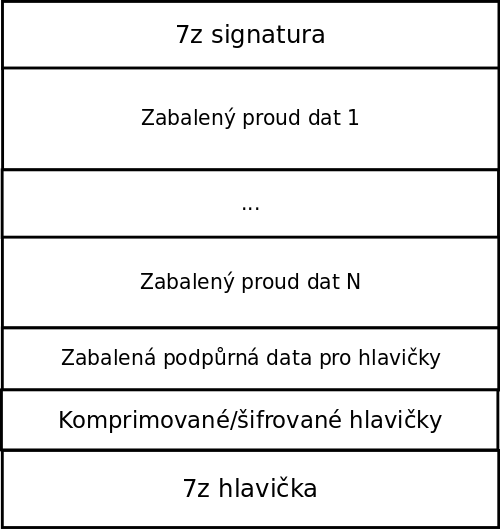
\includegraphics{fig/7z_structure}
	}
    \end{center}
    \caption{Struktura .7z souboru \cite{Pavlov:2015}}
    \label{7zstruct}
\end{figure}
Pro účely této práce nás především zajímá hlavička {\it 7zHeader} a~v~ní obsahy položek nesoucích
informace o~proudech dat (0x03 nebo 0x04). V~nich konkrétně položka informace o~kóderech (0x07),
ve které se musíme propracovat k~poli bajtů {\it CodecInfo}. Hodnoty tohoto pole musíme otestovat
a zjistit, zda se shodují s~identifikátorem standardní šifrovací metody AES-256 + SHA-256
[0x06, 0xF1, 0x07, 0x01]~\cite{Pavlov:2015}. Zde je třeba také nálezt data o použité kompresi.
Kompresní metoda LZMA má identifikátor [0x03, 0x01, 0x01]. Další důležitou položkou pro ověření hesla je CRC šifrovaného souboru. 

Tento typ archivu bohužel neobsahuje žádnou jinou metodu ověření hesla než pomocí spočítání a
porovnání CRC hodnot. K tomu je nutné nejprvek celý soubor dešifrovat a dekomprimovat což značně
přidává na náročnosti celého ověřovacího procesu.

\section{Srovnání}
Pokud budeme srovnávat formáty z~pohledu komprese, zjistíme, že .7z je dle měření efektivnější
než
.ZIP\footnote{\url{http://www.howtogeek.com/200698/benchmarked-whats-the-best-file-compression-format/}}. Ovšem nás spíše zajímá zabezpečení.

 Šifrování formátu .ZIP metodou PKZIP nemá smysl ani porovnávat s~ostatními, neboť se jedná
o~metodu, která již nedostačuje dnešním bezpečnostním standardům~\cite{PKWARE:2014}. 

 Pokud se ale podíváme na silnější metody zabezpečení, zjistíme, že formáty jsou z~hlediska
bezpečnosti vyrovnané. Oba dva podporují AES-256 s~využitím nějaké hešovací metody pro zabezpečení
hesla. Oba formáty také podporují šifrování hlaviček obsahujících informace o~metodách, které jsou
používány a~jaké soubory obsahují.

 Formát .ZIP překonává .7z možností použití elektronických podpisů (certifikát typu X.509v3)
k~šifrování souborů namísto hesel. 7z tuto funkcionalitu vůbec neobshahuje. 



\chapter{Návrh modulů}
\label{ch:moduly}
V~této kapitole se podíváme na to, jak z~výše popsaných algoritmů, technologií a~strukturálních
analýz archivů vytvoříme rozšiřující moduly pro nástroj Wrathion. Tato kapitola si klade za cíl
obecně popsat, jak se budou soubory jednotlivých formátů procházet. Tedy jaká data se z~nich budou
číst, jaké operace je potřeba provést nad vygenerovanými hesly a~jak se bude provádět ověřování
shody hesel.

\section{Modul ZIP}
Jako první si nastíníme modul ZIP. Nemusíme zde řešit návrh celého modulu a~všech
možností pro formát, ale pouze rozšíření funkcionality o~zatím nepodporavané metody zabezpečení.

 Momentální verze ZIP modulu podporuje pouze staré šifrování PKWARE a~šifrování AES. Podpora
šifrování AES je však neúplná. Modul momentálně podporuje pouze speciální verzi AES, jež si
vytvořili vývojáři nástroje WinZip. Ti si vytvořili vlastní ořezanou AES hlavičku a~označili
soubor vlastní metodou. Existují ovšem nástroje jako SecureZIP od firmy PKWARE umožňující také
zašifrovat obsah archivů pomocí šifrovací metody AES, s~níž si současný modul i~přes podporu
zjištění hesla pro AES neporadí.

 Další šifrovací metodou, kterou nabízí nástroj SecureZIP je 3DES. S~ním si momentální verze
neporadí vůbec a~je tedy vhodné tuto funkcionalitu doplnit.

\subsection{Zjištění informací z~archivu}
Následující text popisuje postup získávání a~zpracování informací nutných pro rozhodnutí, zda se
jedná o~ZIP soubor, zda je soubor šifrován, jakou metodou je šifrován, jaké jsou inicializační
hodnoty použité při šifrování apod. To vše je potřeba pro rozšíření funkcionality modulu. Popis se
primárně nesoustředí na získání dat pro již implementované funkce, ale pouze dat důležitých pro
rozšíření funkcionality modulu (detailní popis hlaviček a~hodnot v~nich je
v~sekci~\ref{ssec:zip_struct}):
\begin{enumerate}
    \item Zjištění signatury -- podíváme se na první 4 bajty a~porovnáme je se signaturou [0x50,
	0x4B, 0x03, 0x04]. Tím ověříme, zda se jedná o~ZIP soubor.
    \item Přečtení {\it General purpose bit flag} -- hodnotu příznaků získáme z lokální hlavičky
	prvního souboru.
    \item Analýza příznaků -- zjišťujeme zda jsou nastaveny první a~sedmý bit příznaků na hodnotu
	1. Pokud nalezneme šifrování u~jednoho souboru předpokládáme, že všechny ostatní soubory
	jsou taktéž šifrované a~že byla použita stejná šifrovací metoda. Pokud je nastaven i~13.
	bit musíme provést čtení dešifrovací hlavičky archivu a~pomocí ní dešifrovat celou
	strukturu centrálního adresáře. Postup dešifrování je identický s~dešifrováním souborů.
    \item Přečtení {\it Compression method} -- z~některé z~hlaviček %\footnotemark[\value{footnote}] 
	souboru. Tato položka nás zajímá, pouze pokud byly bity jedna a~sedm příznaků nastaveny na
	hodnotu 1. Číslo uvedené v~této položce nám dovoluje zjistit, zda byla použita šifrovací
	metoda WinZip AES (hodnota 99). Použití jiné hodnoty indikuje použití některé z~dalších
	šifrovacích metod definovaných ve specifikaci formátu .ZIP~\cite{PKWARE:2014}.
    \item Přečtení {\it Extra fields} -- potřebujeme najít hlavičku s~daty o~šifrování, která se
	může vyskytnout pouze za hlavičkou souboru v~centrálním adresáři. V~tomto kroku zjistíme
	informace o~použité šifrovací metodě, délce klíče atd.
    \item Získání hodnot hlavičky pro dešifrování -- nachází se před uloženými daty souboru.
	Potřebujeme získat použitá inicializační data potřebná pro šifrovací s~dešifrovací funkce.
	A~také data pro ověření hesla včetně jejich kontrolního součtu (CRC32).
\end{enumerate}
Jakmile takto získáme všechna potřebná data, přesuneme se k~hledání použitého hesla. Tento proces
bude možné realizovat za využití CPU nebo GPU. Pro obě tato zařízení je nutné vytvořit samostatný
kód. Kód pro CPU čistě v~jazyce C++ s~možností využití některých již implementovaných funkcí a
generátorů obsažených v~nástroji Wrathion. Pro GPU je třeba vytvořit kód v~C++, který poběží na
CPU a~bude inicializavat GPU a~rozdělovat práci pracovním jednotkám na ní umístěných a~poté kernel
v~OpenCL pro implementování kernelu, který poběží na pracovních jednotkách. Avšak v~obou
případech půjde o~totožný Algoritmus~\ref{alg:zip_ver}.

\begin{algorithm}[ht]
    \SetStartEndCondition{ (}{)}{)}\SetAlgoBlockMarkers{}{}%
    \SetKwFor{For}{for}{\string:}{}%
    \SetKwIF{If}{ElseIf}{Else}{if}{}{else if}{else}{}%
    \SetKwRepeat{Repeat}{repeat}{until}%
    \SetKwInOut{Input}{vstup}\SetKwInOut{Output}{výstup}
    \AlgoDisplayBlockMarkers\SetAlgoNoLine%
    \DontPrintSemicolon
    \Input{Data získaná z~hlavičky pro dešifrování (IV, Erd, Dlen, Data)}
    \Output{Poslední vygenerované heslo}
    \Repeat{$ CRC != spocitejCRC32 (Data, Dlen-4) $}{
	heslo = generujHeslo ()\;
	odvozene\_heslo = odvodHeslo (SHA1(heslo))\;
	rd = desifruj (Erd, odvozene\_heslo, IV)\tcc*{Random hodnota pro šifrování}
	odvozene\_heslo = odvodHeslo (SHA1(rd + IV))\;
	desifrovana\_data = desifruj (Data, odvozene\_heslo, IV)\;
	CRC = *(uint32*)(\&Data[Dlen-4])\tcc*{Poslední 4 bajty jsou CRC}
    }
    \caption{Princip ověření vygenerovaného hesla pro ZIP archiv}\label{alg:zip_ver}
\end{algorithm}

\section{Modul SevenZ}
V~tomto případě se jedná o~úplně nový modul. Bude tedy potřeba nadefinovat všechny struktury
potřebné k~provozu modulu v~rámci nástroje Wrathion a~implementovat metody šifrování, hešování,
odvozování hesel a~jiné používané formátem .7z.

\subsection{Zjištění informací z~archivu}
Archiv formátu .7z v~sobě, stejně tak jako .ZIP archiv, nese informace nutné pro umožnění
dešifrování souboru. V~tomto případě je však o~něco složitější je získat. Struktura 7z archivu
je hodně komplexní a~proměnlivá. Struktura hlaviček do značné míry připomíná databázi. Pro
detailní porozumění struktuře řídících dat formátu je třeba nahlědnout do souboru
7zFormat.txt~\cite{Pavlov:2010}. Potřebné informace lze získat následujícím značně zjednodušeným
teoretickým postupem:
\begin{enumerate}
    \item Ověříme signaturu -- jedná se o~prvních 6 bajtů souboru, které musí odpovídat hodnotě
v~sekci \ref{ssec:7z_struct}. 
    \item Přejdeme na pozici 6 bajtů za signaturou, kde	prvních 8 bajtů obsahuje pozici hlavičky.
	Na dalších 8 bajtech je délka hlavičky.
    \item Přejdeme na začátek hlavičky.
    \item Přejdeme na záznam se signaturou 0x06, ze kterého získáme pozici dat k níž přičteme 32.
    \item Přejdeme na záznam se signaturou 0x09, ze kterého získáme délku proudu dat.
    \item Přejdeme na záznam se signaturou 0x0B, ve kteté hledáme hodnoty [0x06, 0xF1, 0x07, 0x01]
	a [0x03, 0x01, 0x01] značící 7zAES a LZMA.
    \item Získáme z nich data -- inicializační vektor, počet iterací použití SHA256 (defaultně
	19) pro 7zAES a inicializační data slovníků pro LZMA.
    \item Přejdeme na záznam se signaturou 0x0A, ze kterého získáme CRC dat souboru.
\end{enumerate}
Jakmile tato data získáme můžeme se přesunout k hledání hesla. Tento proces, popsáný
Algoritmem~\ref{alg:7z_desifr}, lze plně realizovat pouze na CPU. Formát 7z totiž může obsahovat
soubory o velké velikosti, které by se nemusely vejít do paměti GPU. Musíme zde vzít totiž v
potaz, že potřebujeme mít v paměti prostor o velikosti souboru pro každou výpočetní jednotku GPU,
na které poběží kernel. Řešení tohoto problému je popsáno v sekci \ref{ssec:7zcrackercpu}.

\begin{algorithm}[ht]
    \SetStartEndCondition{ (}{)}{)}\SetAlgoBlockMarkers{}{}%
    \SetKwFor{For}{for}{\string:}{}%
    \SetKwInOut{Input}{vstup}\SetKwInOut{Output}{výstup}
    \SetKwRepeat{Repeat}{repeat}{until}%
    \AlgoDisplayBlockMarkers\SetAlgoNoLine%
    \DontPrintSemicolon
    \Input{Data získaná z~hlaviček}
    \Output{Poslední vygenerované heslo}
    \Repeat{$ CRC != spocitejCRC32 (data) $}{
	heslo = generujHeslo ()\;
	klic = derivuj\_heslo(heslo, iteraci)
	desif\_data = desifruj\_data(klic, IV, sif\_data)
	data = dekomprimuj(desif\_data, lzma\_data)
    }
    \caption{Princip vytvoření hesla pro dešifrování pomocí 7z}\label{alg:7z_desifr}
\end{algorithm}
    
\chapter{Implementace}
\label{ch:implementace}
Tato kapitola se věnuje popisu implementace přidáné funkcionality modulu ZIP a nového modulu pro
7z do nástroje Wrathion. Jsou v ní také zmíněny použité knihovny a verze použitých knihoven
implementujícíh dešifrovací a dekomprimační metody. Kapitola je rozdělena do dvou částí, každá
reprezentující jeden z formátů jimiž se tato práce zabývá.

\section{Implementace modulu ZIP}
Jak již bylo zmíněno tento modul bylo třeba pouze obohatit o určité nedostatky, které se týkaly
především podpory metod šifrování. Konktrétně se jedná o metody šifrování souborů AES a DES a také
o metodu umožňující šifrování {\textit Central Directory} záznamu. Tyto metody jsou definované ve
standardu formátu ZIP vydaném firmou PKWARE v rámci APPNOTE.txt~\cite{PKWARE:2014} a používány v
nástrojích z rodiny SecureZIP od PKWARE.

\subsection{ZIPFormat}
Tato třída slouží ke čtení potřebných informací z archívu na vstupu. Získává tedy imformace o tom
jaká šifrovací metoda byla použita na základě čehož pak hledá další pro nás důležitá data ve
struktuře souboru. Data jsou ukladána do struktury $ZIPInitData$, která je použita pro
inicializaci nových instancí tříd crackerů. 

 Třída byla upravena tak, aby byla schopna detekovat výše zmíněné metody a uložit data potřebná pro
následné ověřování hesel.

\subsection{ZIPStAESCrackerCPU}
Jedná se o třídu s implementací pro ověření hesla metodou AES čistě na CPU. Třída obsahuje funkci
pro ověření hesla $checkPassword()$ a funkce $derive()$, $derive\_key()$ a $sha1()$ pro vytvoření
šifrovacích klíčů.

 Třída využívá implementace šifrovací funkce AES použité v nástroji UnRAR, kde je
implementována jako třída Rijndael pod licencí Public Domain. Datové typy použíté v převzaté
třídy byly pozměny tak, aby odpovídaly typů používaným v našem nástroji.
 
 Obě derivační funkce vytvářejí blok, který odpovídá funkci $CryptDeriveKey()$ z MS
CryptoAPI~\cite{CryptoAPI}. Funkce $sha1()$ je převzata z dříve implemetovaných částí modulu ZIP.

 Funkce $checkPassword()$ implementuje algoritmus \ref{alg:zip_ver} jenž slouží k ověření hesla
získaného z generátoru. Algoritmus je odvozen algoritmu uvedeného v APPNOTE.txt začínajícího na
řádku 2720.

\subsection{ZIPStAESCrackerGPU}
Tato třída obsahuje implementaci pro ověření hesla metodou AES na GPU. Tato třída slouží pouze k
vytvoření, inicializování a předání paměťových objektů (zásobníků) OpenCL kernelu
$zip\_staes\_kernel$. To je realizováno ve funkci $initData()$. 

 K ověření hesla je realizováno GPU kernelem. Na CPU se po zjištění nálezu provede pouze
kontrola voláním funkce $verifyPassword()$. Tato funkce využívá objektu s typem třídy
$ZIPStAESCrackerCPU$ a volání jeho funkce $checkPassword$, která je volá s kernelem označeným
heslem na vstupu.

\subsubsection{zip\_staes\_kernel}
Kernel je na napsán v jazyce OpenCL C jeho funkcionalita odpovídá funkce $checkPassword()$ ze
třídy $ZIPStAESCrackerCPU$. Implementačně je zde jeden znatelný rozdíl. Dynamické vytváření Sbox
tabulek pro AES je nahrazeno konstantními tabulkami.
 
\subsection{ZIPTDESCrackerCPU}
Jedná se o třídu obsahující pokus o implementaci metody 3DES pro CPU. Jedná se o třídu velmi
podobnou třídě $ZIPStAESCrackerCPU$. Jediným rozdílem je funkcí pro 3DES z knihovny OpenSSL
namísto funkcí pro AES.

 Tuto třídu se mi bohužel nepovedlo zprovoznit. Příčinu problému s funkčností vidím v přidávání
paritních bitů ke klíči a inicializačnímu vektoru, jenž je knihovnou vyžadováno. Dalším
problémem s laděním tohoto problému je, že se mi nepovedlo nalést ani žádný Open Source
archivační program, který by uměl takovýto soubor dešifrovat. To značně komplikuje proces ladění,
když není možné porovnávat rozdíly v hodnotách v jednotlivých krocích.

\section{Implementace modulu SevenZ}
V tomto případě bylo třeba vytvořit úplně nový modul. K tomu bylo třeba vytvořit soubory {\textit
SevenZModule.cpp, SevenZFormat.cpp} a soubory pro CPU a GPU cracker. Soubory v sobě nesou
stejnojmenné třídy implementující funkce vyžadované pro správnou komunikaci s naším nástrojem.

\subsection{SevenZFormat}
Podobně jako třída $ZIPFormat$ i tato slouží k získání a zpracování informací uložených v
archivu. Pro uložení byla vytvořena struktura $SevenZInitData$ skádající se z položek základních
datových typů, ale také z dalších vytvořených struktur. Mezi ně jmenovitě patří $SevenZCoder$,
$SevenZFolder$ a $SevenZPackInfoHdr$, které reflektují položky obsažené ve struktuře hlavičky
souboru. Tento přístup k uložení dat byl zvolen na základě již zmíněného problému jímž je, že
struktura hlavičky u formátu .7z je značně komplikovaná a proměnná. Čtení struktury ulehčují
odpovídající funkce v této třídě.

 Třída mimo jiné obsahuje funkci $SevenZUINT64()$ implementující dekodér 64 bitových
bezznamýnkových čísel. Tohoto kódování velkých čísel je ve formátu .7z použito k redukování
paměťového prostoru potřebného k uložení takového čísla. Ve zkratce to funguje tak, že počet
jedniček v nepřerušené řadě začínající na nejvyšších pozicích v prvním bajtu určuje kolik
následujících bajtů se ještě váže k tomuto číslu. Zbytek prvního bajtu za prvním výskytem nuly je
použit k uložení hodnoty nejvýznamnějšího bajtu~\cite{Pavlov:2010}. 

\subsection{SevenZCrackerCPU}
\label{ssec:7zcrackercpu}
Tato třída obsahuje implementaci funkcí potřebných pro ověření hesla na CPU. Stejně tak jako
všechny ekvivalentní třídy v ostatních modulech i tato obsahuje funkci $checkPassword()$ a pak
funkce pro vytvoření klíče pro dešifrování a funkci se starající se o samotné dešifrování a
dekompresi dat.

 Funkce pro dešifrování a dekompresi byly převzaty z nástroje 7zip vytvořeného autorem formátu .7z
Igorem Pavlov, tyto funkce vytvořil pod licencí Public Domain. Díky tomu, že nástroj 7zip je
napsán v C / C++ nebylo třeba nijak do funkcí respektive tříd vůbec zasahovat. Funkce $hash()$
vytvářející klíč pro dešifrování byla také značně inspirována zdrojovými kódy 7zip-u. 

 Ve funkci $checkPassword()$ je použita rychlostní optimalizace sloužící k redukci času
potřebného k určení zda se může jedna o správné heslo. Optimalizace funguje následujícím způsobem:
\begin{enumerate}
    \item Zjistíme jestli jsou data pro dešifrování velká alespoň 32 bajtů. Pokud jsou menší tak
	se optimalizace nepoužije.
    \item Vezmeme prvních 16 bajtů dat.
    \item Provedeme nad nimi operaci dešifrování.
    \item Ověříme hodnoty na začátku dešifrovaných dat. Pokud je první bajt roven 0x00
	(pevná první hodnota dat dekomprimovatelnch LZMA) nebo pokud se první tři bajty rovnají
	0x0104006 (posloupnost signatur v hlavičce archivu typu .7z) tak pokracujeme podle
	Algoritmu~\ref{alg:7z_desifr} pro celé data souboru. Jinak heslo zahodíme a jdeme o
	začátku s novým heslem.
\end{enumerate}
\subsection{SevenZCrackerGPU}
Jak již název naznačuje jedná se o třídu s implementací funkce pro inicializaci dat na GPU a s
funkcí pro ověření hesla získaného z GPU. Ačkoliv to vypadá velmi podobně je zde jeden velký
rozdíl v tom, kdy a jak dostaneme správné heslo. S jistou nadsázkou se dá říct, že se jedná o
třídu provádějící obnovení hesla na CPU s jistou formou heuristiky. 

Formout heuristiky jsou kroky 1 - 4 optimalizace popsáné v předchozí podkapitole. Rozdíl oproti
CPU implementaci je ten, že filtrování hesel obstarává GPU a nemusíme ho tedy provádět na CPU.
Teoreticky by nám tímto způsobem filtrování sníží počet hesel zhruba 256-krát v případě, že
šifrovaná data jsou i komprimovaná data. V případě, že se bavíme archivech .7z, které obsahují
pouze jeden soubor a jejich hlavička tedy před šifrováním není komprimovaná, pak se dostáváme
daleko větší redukci hesel.

\subsubsection{sevenz\_aes\_kernel}
Kernel obsahuje přepis tříd převzatých z nástroje 7zip. Jediné modifikace těchto tříd jsou
provedeny nahrazením funkcí pro generování AES a SHA256 tabulek za konstantní tabulky. Kernel jako
takový provádí pouze filtraci hesel pro CPU. 

Důvodem proč neprovádíme všechny kroky na GPU je poměrně jednoduchý. GPU nemá dostatek paměti na
to, aby mohla obsahovat několik instancí dat k dešifrování. V archivu mohou být obsaženy soubory o
velikosti několika gigabajtů a není tedy v naší moci takto velký shluk dat vměstnat. Pokusy o
vměstnání několika instancí takovýchto dat je tedy naprosto nereálné. 

\chapter{Měření a srovnání}
\label{ch:mereni_a_srovnani}
\section{7zip archiv se šifrovanou hlavičkou}
\subsection{Srovnaní s konkurencí}
\section{7zip archiv bez šifrované hlavičky}
\subsection{Srovnaní s konkurencí}
\section{ZIP archiv se šifrovanou hlavičkou}
\subsection{Srovnaní s konkurencí}
\section{ZIP archiv bez šifrované hlavičky}
\subsection{Srovnaní s konkurencí}
\section{7zip archiv s různou velikostí}
\subsection{Srovnaní s konkurencí}
\section{Škálovatelnost modulů}
\subsection{Srovnaní s konkurencí}
\subsection{Srovnaní s konkurencí}
Cil: Zjistit rychlost crackovani 7zip archivu se sifrovanou hlavickou pro ruzne dlouha hesla.
Cil: Zjistit rychlost crackovani 7zip archivu bez sifrovane hlavicky pro ruzne dlouha hesla.
Cil: Zjistit rychlost crackovani ZIP archivu bez sifrovane hlavicky pro ruzne dlouha hesla.
Cil: Porovnat rychlost crackovani 7zip archivu bez sifrovane hlavicky pro ruzne velke soubory.
Cil: Porovnat rychlost crackovani ZIP a 7zip archivu pri pouziti vice grafickych karet.
Cil: Porovnat me moduly a kernely s konkrurenci.

\chapter{Závěr}
Obsáhnout všechny možnosti a~nastavení analyzovaných formátů je značně náročný proces, který
ve většině případů ani nestojí za námahu. Důvodem je nízký počet dostupných nástrojů schopných tyto
hodnoty nastavit, což platí hlavně pro formát ZIP.

 Struktury jednotlivých formátů byly popsány tak, aby bylo možné chybějící nebo nejasné informace
dohledat ve specifikacích formátu a~nebylo nutné složitě hledat, o~jaké hodnoty se jedná. Zde
je nutno podotknout, že, jak již bylo zmíněno, struktura 7z souboru je hodně komplexní a~proměnná.
Bohužel dokumentace tohoto formátu je značně nedostačující a~je tedy nutné strávit hodně času
studiem struktury, zdrojových kódů a~fóra vývojáře pro získání dalších a~detailnějších informací.

 Návrh rozšíření modulu pro ZIP by měl z~většiny odpovídat tomu, jak bude rozšíření vypadat po jeho
implementaci. Také na základě průzkumu v~tomto odvětví by rozšířený modul měl být napřed před
konkurencí. Některé známé nástroje totiž mají podporu pouze pro WinZip AES a~PKWARE šifrování
(John the Ripper) nebo momentálně neposkytují funkcionalitu k~formátu .ZIP (oclHashcat).  

 U~modulu 7z se jedná spíš o~teoretický nástin, jak by mohl modul vypadat a~jak by
mohly jednotlivé části algoritmu fungovat. Některé důležité informace totiž nejsou nikde detailně
popsány. Hledání informací ve zdrojových kódech 7zip-u je díky absenci komentářů a~vysoké
abstrakci kódu značně náročné a~zdlouhavé. Návrh modulu bude tedy potřeba pravděpodobně
modifikovat na základě informací zjištěných během implementace jednotlivých částí modulu.

 Během implementace bude zapotřebí vytvořit dvě verze obou modulů. Jednu verzi běžící pouze na
CPU a~druhou, která bude podporovat paralelní zpracování na GPU. V~návaznosti na implementaci
bude potřeba provést měření rychlosti a~srovnání s~dalšími nástroji. Podle výsledků srovnání
jde odhadnout, jak moc optimální náš modul je a~zda je potřeba jej upravit a~vyladit nebo
zda je v~rámci možností optimalizován.


Doplnit: Wrathion by sel rozsirit o moznost zasilat z GPU i hashe do CPU pro false positive hesla
u 7z. Cimz by se 7z Crackovani urychlilo. Taky by bylo dobry provade kontrolu false positive hesel
ve vice vlaknech aby se to urychlilo.

%=========================================================================
